
\documentclass{beamer}


\mode<presentation>
{
  \usetheme{Rochester}
  \setbeamercovered{transparent}
}


\usepackage[english]{babel}
\usepackage[utf8]{inputenc}
\usepackage{times}
\usepackage[T1]{fontenc}

\title[Short Paper Title] % (optional, use only with long paper titles)
{Efficient and Robust Automated Machine Learning}

%\subtitle
%{Include Only If Paper Has a Subtitle}

\author[Author] % (optional, use only with lots of authors)
{Bucevschi Alexandru\inst{1} and Stoleru Ingrid\inst{1}}
% - Give the names in the same order as the appear in the paper.
% - Use the \inst{?} command only if the authors have different
%   affiliation.

\institute[Universities of Somewhere and Elsewhere] % (optional, but mostly needed)
{
  \inst{1}
  Facultatea de Informatica\\
  Universitatea "Alexandru Ioan Cuza"
}
% - Use the \inst command only if there are several affiliations.
% - Keep it simple, no one is interested in your street address.

\begin{document}

\begin{frame}
  \titlepage
\end{frame}

\begin{frame}{Outline}
  \tableofcontents
  % You might wish to add the option [pausesections]
\end{frame}

\section{Prezentarea subiectului}

\subsection{Automated Machine Learning}
\begin{frame}{AutoML}
	\begin{center}
		\textbf{Automatizarea procesului de aplicare a abordarilor de ML in problemele de zi cu zi.}
	\end{center}
\end{frame}

\begin{frame}{AutoML - problemele adresate}
	\begin{center}
		\begin{itemize}
			\item Detectia automata a tipurilor datelor de intrare
			\item Determinarea automata a task-ului: clusterizare, clasificare binara/ multi-class
			\item Automatizarea procesului de feature engineering (selection/extraction)
			\item Selectarea automata a modelului
			\item Optimizarea automata a hiperparametrilor
		\end{itemize}
	\end{center}
\end{frame}


\begin{frame}{Subiectul paper-ului}
	\begin{center}
		Paper-ul curent propune un nou sistem de \textbf{AutoML}, intitulat AUTO-SKLEARN.\\
		\vspace{0.5cm}
		Acesta este bazat pe \textbf{scikit-learn}:
		\vspace{0.25cm}
		\begin{itemize}
			\item machine learning library (Python)
			\item 15 clasificatori
			\item 14 metode de feature preprocessing
			\item 4 metode de data preprocessing
		\end{itemize}
	\end{center}
\end{frame}

\begin{frame}{Avantajele sistemului propus}
		\begin{center}
			Ia in calcul in mod automat performantele anterioare pe dataset-uri similare si construieste ensemble-uri din modelele evaluate la faza de optimizare.
		\end{center}
\end{frame}


\subsection{Formularea problemei}
\begin{frame}
	\begin{center}
		\textbf{Problema AutoML}:\\
		Producerea automata (fara interventia utilizatorului) a predictiilor pentru un set nou de date, intr-un buget computational fix.\\
		\vspace{0.5cm}
		\textbf{Buget computational} = Memorie, CPU
	\end{center}
\end{frame}

\begin{frame}
	\begin{figure}[H]
	\centering
	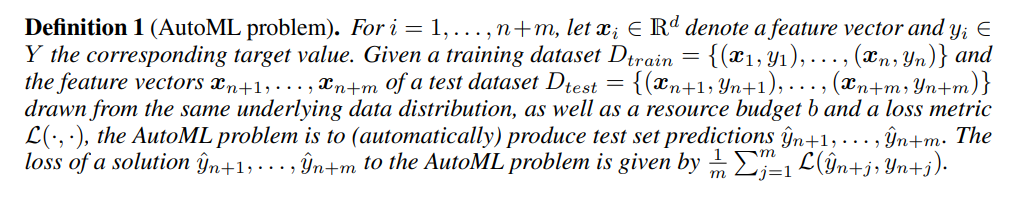
\includegraphics[scale=0.5]{formula_automl.PNG}
	\end{figure}
\end{frame}

\section{AutoML modelata ca o problema CASH}

\begin{frame}{Probleme AutoML}
	\begin{center}
		\begin{itemize}
			\item Niciun algoritm individual de ML nu performeaza foarte bine pe toate seturile de date.
			\item Unele abordari de ML se bazeaza pe optimizarea de hiperparametri (SVM-ul non-linear). 
		\end{itemize}
	\end{center}
\end{frame}


\begin{frame}{Combined Algorithm Selection and Hyperparameter optimization}
	\begin{figure}[H]
		\centering
		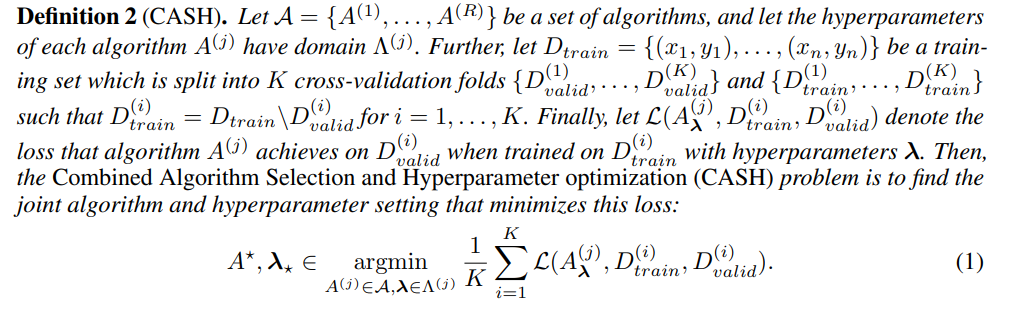
\includegraphics[scale=0.5]{formula_cash.PNG}
	\end{figure}
\end{frame}


\begin{frame}{CASH - Aim}
	\begin{center}
		Incercam sa identificam o combinatie de algoritmi din tot spatiul de algoritmi, cu hiperparametrii corespunzatori, care performeaza cel mai bine pe toate seturile de date. \\
		(Minimizeaza functia de loss, deci numarul de instante clasificate gresit)
	\end{center}
\end{frame}

\begin{frame}{CASH - Aim}
	\begin{figure}[H]
		\centering
		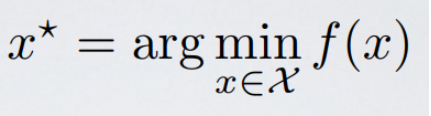
\includegraphics[scale=0.75]{optim.PNG}
	\end{figure}
\end{frame}


\begin{frame}{CASH - Blackblox}
	\begin{itemize}
		\item Nu avem gradientii functiei
		\item Evaluarea functiei este costisitoare
		\item Optimizarea - Strategie secventiala (colectam date, apoi pe baza lor decidem ce punct vom evalua in continuare)
	\end{itemize}
\end{frame}

\subsection{Optimizarea Bayesiana}
\begin{frame}{Solutie}
	\begin{center}
		\textbf{Optimizarea Bayesiana}
	\end{center}
		\begin{itemize}
			\item Metoda iterativa
			\item Tine cont de evaluarile din trecut, formand un model probabilistic 
			\item Mapeaza hiperparametrii la probabilitatea de a obtine un anumit scor
		\end{itemize}
\end{frame}

\begin{frame}{Optimizarea Bayesiana}
	\begin{figure}[H]
		\centering
		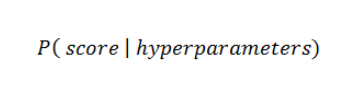
\includegraphics[scale=0.75]{prob.PNG}
	\end{figure}
\end{frame}

\begin{frame}{Optimizarea Bayesiana}
	\begin{itemize}
		\item "Surogatul functiei obiectiv"
		\item Mai usor de optimizat decat functia obiectiv
		\item Selecteaza hiperparametrii care performeaza cel mai bine pe functia surogat
		\item Calculeaza valoarea functiei obiectiv si face update la surogat
	\end{itemize}
\end{frame}

\begin{frame}{Optimizarea Bayesiana}
	\begin{center}
		\textbf{"Spend a little more time selecting the next hyperparameters in order to make fewer calls to the objective function."}
	\end{center}	
\end{frame}

\subsection{Modelul propus}
\begin{frame}{Avantajele modelului propus}
	\begin{figure}[H]
		\centering
		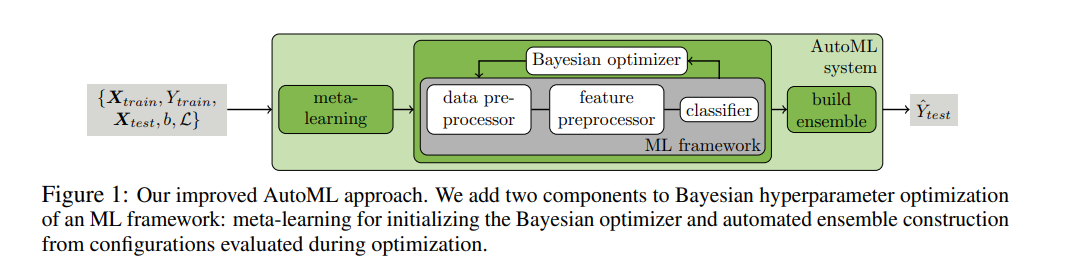
\includegraphics[scale=0.5]{conf.PNG}
	\end{figure}
\end{frame}

\section{Elementul de noutate}
\subsection{Meta-learning pentru selectarea instantierilor de framework}

	\begin{frame}{Complementaritatea}
		\begin{itemize}
			\item Meta-learning-ul sugereaza instantieri ale framework-ului care sunt probabile sa performeze bine
			\item Optimizarea bayesiana realizeaza fine-tuningul pe partea de performanta 
		\end{itemize}	
	\end{frame}

	\begin{frame}{Imaginea de ansamblu}
		\begin{itemize}
			\item Se selecteaza k configurari pe baza meta-learningului
			\item Se initializeaza un algoritm de optimizare bayesiana cu aceste configurari
		\end{itemize}	
	\end{frame}

	\begin{frame}{Generarea configuratiilor initiale}
		\begin{itemize}
			\item S-a pornit de la repo-ul de OpenML - \textbf{140 dataseturi}
			\item S-au implementat 38 de meta-feature-uri, ce caracterizeaza dataseturile
			\item Exemple de feature-uri:
				\begin{itemize}
					\item Statistici despre numarul de instante, feature-uri si clase
					\item Entropia label-urilor
					\item Data skewness
				\end{itemize}			
		\end{itemize}	
	\end{frame}

	\begin{frame}{Meta Learning}
		\begin{itemize}
			\item Pentru fiecare dataset, s-au evaluat feature-urile
			\item A fost folosita optimizarea bayesiana pentru a determina o instantiere a frameworkului cu rezultate foarte bune pe acel dataset.
		\end{itemize}	
	\end{frame}

	\begin{frame}{Evaluarea pe un dataset nou}
		\begin{itemize}
			\item Se calculeaza meta-feature-urile
			\item Se calculeaza distanta L1 fata de celelalte dataset-uri in spatiul de feature-uri
			\item Se aleg cele mai apropiate 25 de dataset-uri si se stocheaza instantierile corespunzatoare, care sunt date optimizatorului
		\end{itemize}	
	\end{frame}

\subsection{Constructia automata de ansambluri din modelele evaluate la faza de optimizare}

	\begin{frame}{Problema optimizarii bayesiene}
		\begin{center}
			O procedura ce consuma resurse utile, in sensul in care modelele care performeaza aproape la fel de bine ca cel mai bun sunt pierdute. 
		\end{center}	
	\end{frame}

	\begin{frame}{Solutia}
		\begin{center}
			Stocheaza cele mai performante modele si printr-o serie de preprocesari, construieste un ansamblu din acestea.
			\begin{itemize}
				\item Robustete
				\item Reducerea overfitting-ului
			\end{itemize}
		\end{center}	
	\end{frame}

	\begin{frame}
		\begin{itemize}
			\item Weight-urile uniforme asociate modelelor individuale nu au condus la rezultate bune.
			\item Metoda optimizata de construire a ansamblurilor - \textbf{ensemble selection}.
			\item Pornim de la un empty ensemble si in mod iterativ adaugam modele care maximizeaza performanta ansamblului la validare. 
			\item Modelele sunt adaugate cu weighturi uniforme, insa se permit repetitiile.
			\item Dimensiunea ansamblului: \textbf{50}
		\end{itemize}
	\end{frame}

\section{Componenta practica a sistemului}

	\begin{frame}{Sisteme}
		\begin{itemize}
			\item Porneste de la \textbf{scikit-learn} - ML library
			\item AUTO-WEKA (optimizarea bayesiana)
			\item AUTO-SKLEARN
		\end{itemize}
	\end{frame}

	\begin{frame}{Exemple}
		\begin{itemize}
			\item Bayes Naiv, Arbori de decizie, KNN, SVM, AdaBoost
		\end{itemize}
		
		\begin{itemize}
			\item PCA, ICA, Polynomial
		\end{itemize}

		\begin{itemize}
			\item One-hot encoding, balansare, rescalare
		\end{itemize}
	\end{frame}
	
	\begin{frame}{Spatiul de configurare}
		\begin{figure}[H]
			\centering
			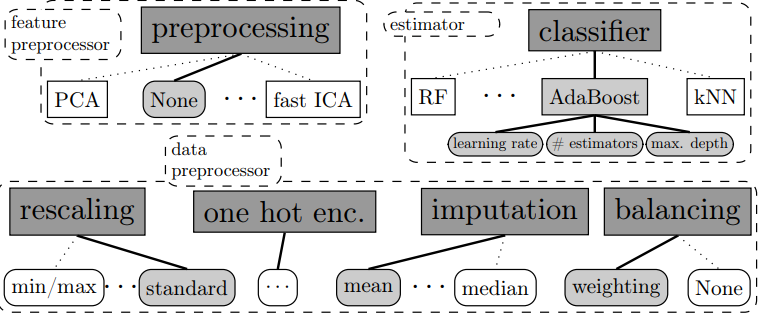
\includegraphics[scale=0.6]{pipeline.PNG}
		\end{figure}	
	\end{frame}


	\begin{frame}{}
		\begin{figure}[H]
			\centering
			
\includegraphics[scale=0.7]{multumesc.PNG}
		\end{figure}	
	\end{frame}


\end{document}
